\documentclass{standalone}
\usepackage{tikz}
\begin{document}
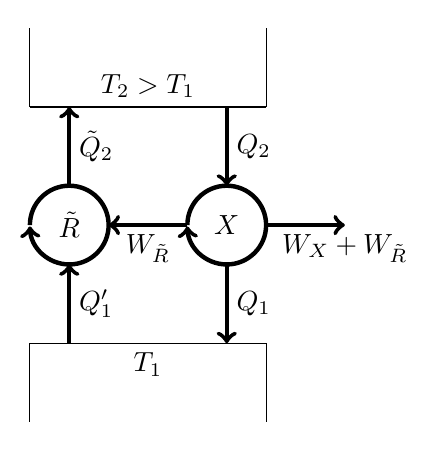
\begin{tikzpicture}[scale=2]
    \draw[-](0.5,0)--(2,0);
    \draw[-](0.5,0)--(0.5,-0.5);
    \draw[-](2,0)--(2,-0.5);

    \node[below]at(1.25,0){$T_1$};

    \draw[->,ultra thick](0.75,0)--(0.75,0.5);
    \node[right]at(0.75,0.25){$Q_1'$};
    
    \draw[->,ultra thick](0.5,0.75)arc(180:-178:0.25);
    \node[]at(0.75,0.75){$\tilde{R}$};

    \draw[->,ultra thick](0.75,1)--(0.75,1.5);
    \node[right]at(0.75,1.25){$\tilde{Q}_2$};

    \draw[->,ultra thick](1.5,0.75)arc(180:-178:0.25);
    \node[]at(1.75,0.75){$X$};

    \draw[->,ultra thick](1.75,0.5)--(1.75,0);
    \node[right]at(1.75,0.25){$Q_1$};
    \draw[->,ultra thick](1.75,1.5)--(1.75,1);
    \node[right]at(1.75,1.25){$Q_2$};

    \draw[->,ultra thick](2,0.75)--(2.5,0.75);
    \node[below]at(2.5,0.75){$W_X+W_{\tilde{R}}$};

    \draw[<-,ultra thick](1,0.75)--(1.5,0.75);
    \node[below]at(1.25,0.75){$W_{\tilde{R}}$};

    \draw[-](0.5,1.5)--(2,1.5);
    \draw[-](0.5,1.5)--(0.5,2);
    \draw[-](2,1.5)--(2,2);

    \node[above]at(1.25,1.5){$T_2>T_1$};
\end{tikzpicture}
\end{document}